\section{Casing \& Protection}
We decided to think about the protection of the components of the nodes and of the central so we started to design different types of boxes on Autodesk Inventor with the intention of 3D printing it.

\subsection{Central Box}
First, we created the frame for the central, it should protect the borders of the screen and the components in a way to improve their lifespan and to give a better design to the central.
\begin{figure}[H]
    \centering
    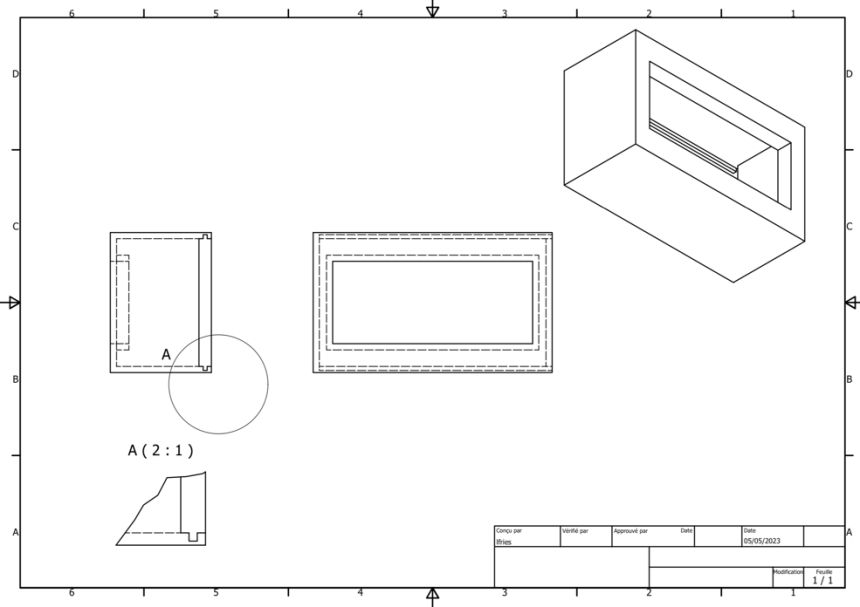
\includegraphics[width=.8\textwidth]{images/casing/img16.jpg}
    \caption{Plan of the frame for the screen}
\end{figure}

--- Step-by-Step Construction

First, we draw a rectangle with another rectangle hole in the middle of the first one. This hole will receive the screen of the central. We give the external rectangle a thickness of 3mm and then we create the walls of the box, they will have the same thickness as the first rectangle.

\begin{figure}[H]
    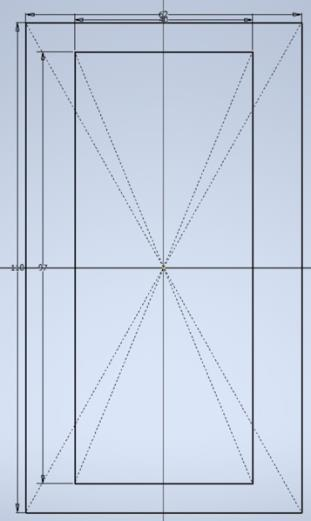
\includegraphics[height=7.5cm]{images/casing/img17.jpg}
    \hfill
    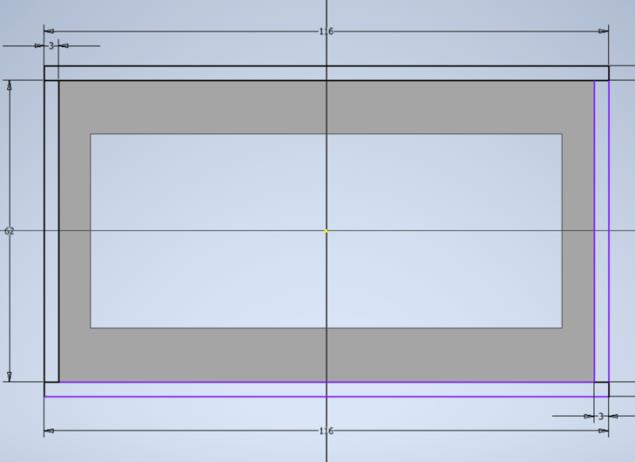
\includegraphics[height=7.5cm]{images/casing/img18.jpg}
\end{figure}

This box has to be high enough to contain all the components of the central so we decided to make it approximately 40mm high.
\begin{figure}[H]
    \centering
    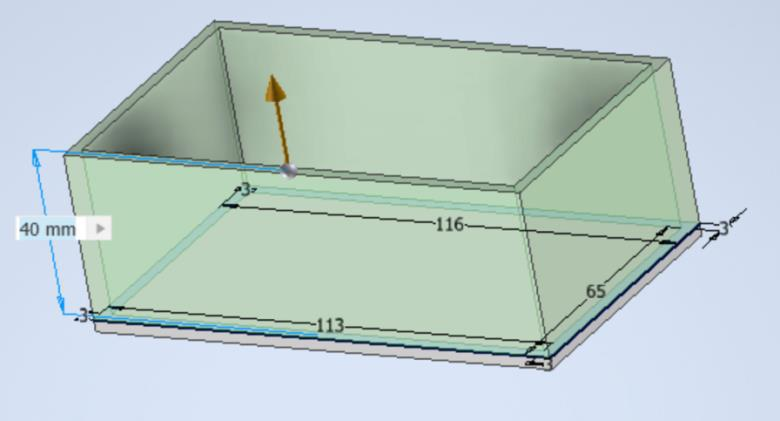
\includegraphics[width=.7\textwidth]{images/casing/img21.jpg}
\end{figure}

We also decided to integrate the screen as cleanly as possible, so we had to create elevations around the screen hole to put the screen at the same level as the front wall of the box. This way, the screen will be better protected and it will have a nicer design.
\begin{figure}[H]
    \centering
    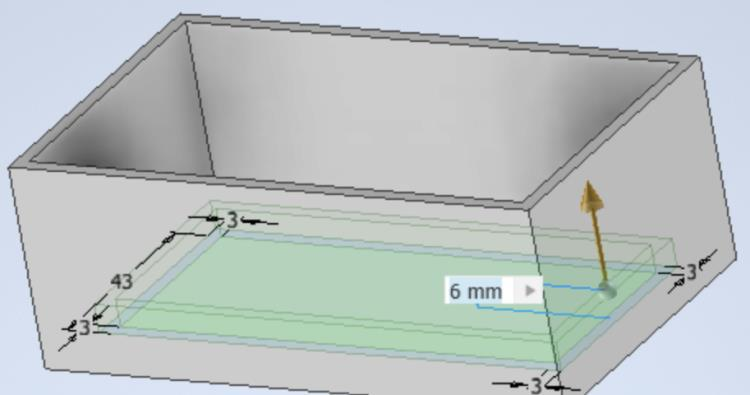
\includegraphics[width=.7\textwidth]{images/casing/img22.jpg}
\end{figure}

The last question about this box was "How to close it ?", to answer this question we decided to create a cover that would slide just behind the box and will remain tightly closed as we have left a fairly tight space.
\begin{figure}[H]
    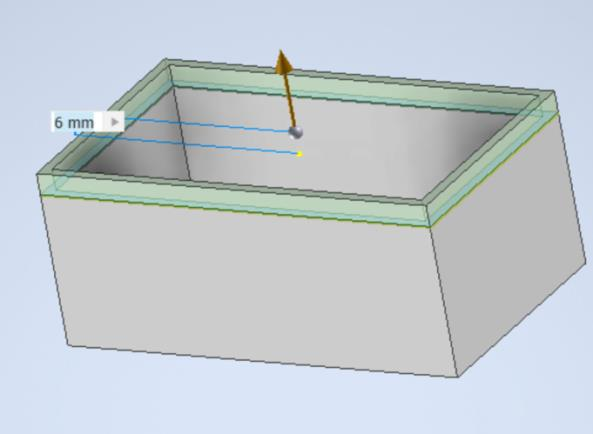
\includegraphics[height=6cm]{images/casing/img23.jpg}
    \hfill
    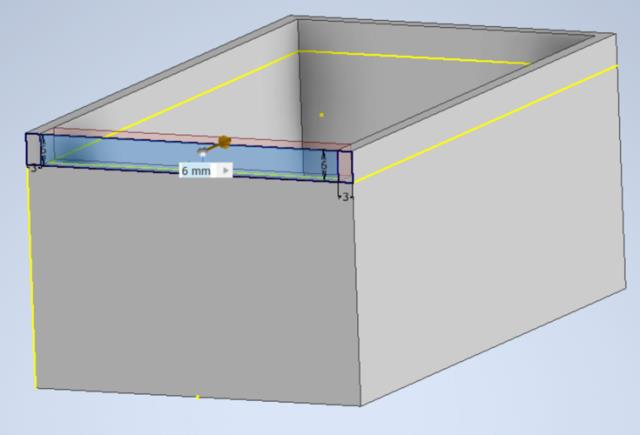
\includegraphics[height=6cm]{images/casing/img24.jpg}
\end{figure}

To let enough space for the cover and for the components, we had to enlarge a bit the box and to create an opening on one side. Finally, we had to create slits on both sides of the box to let the cover slide in its space.
\begin{figure}[H]
    \centering
    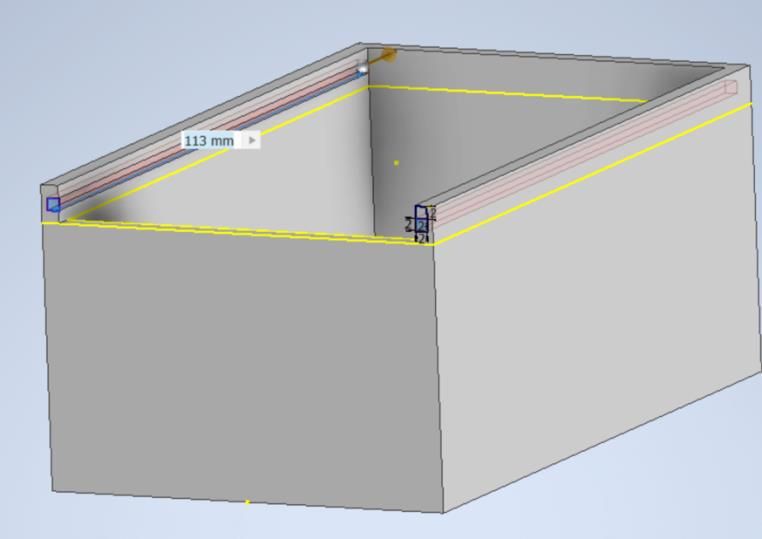
\includegraphics[width=.7\textwidth]{images/casing/img27.jpg}
\end{figure}

When we finished the design of the box we had to think about the design of the cover. We decided to create a simple board that could slip in and out of its space.
\begin{figure}[H]
    \centering
    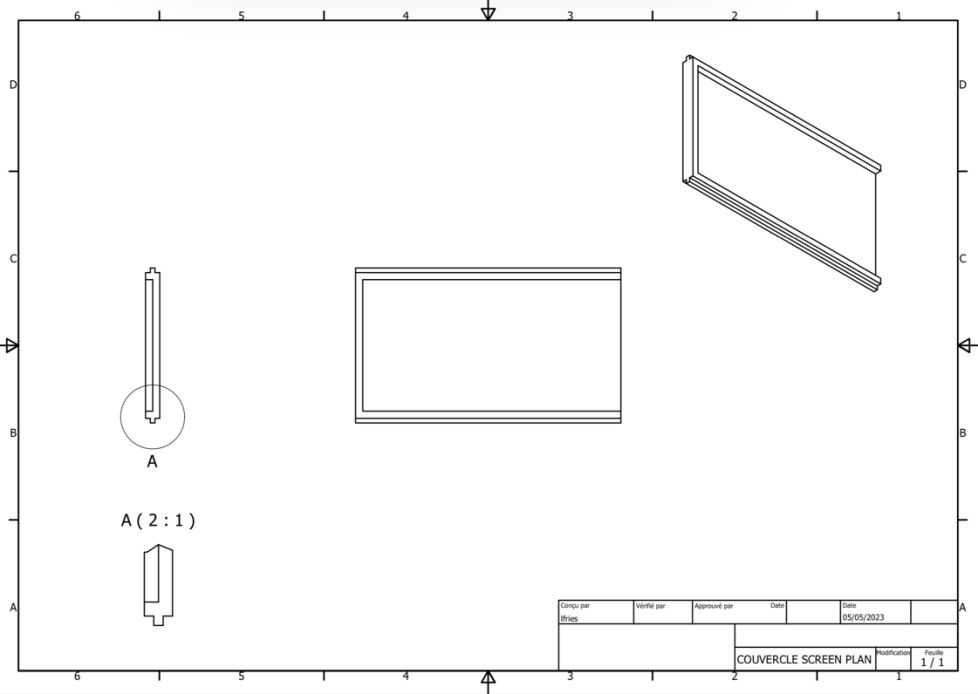
\includegraphics[width=.7\textwidth]{images/casing/img28.jpg}
    \caption{Plan of the cover of the central}
\end{figure}

To make this cover, we first started to create a rectangle of the right dimensions and we gave this rectangle a thickness of 3 mm. Then, we also added 3 mm to the sides of this rectangle so it can correctly close the box.
\begin{figure}[H]
    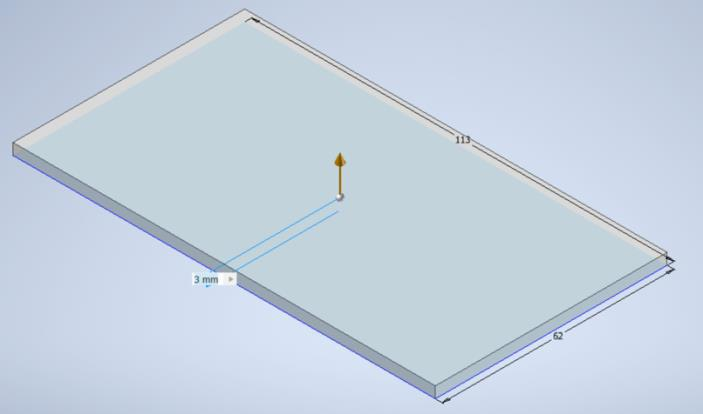
\includegraphics[height=5cm]{images/casing/img31.jpg}
    \hfill
    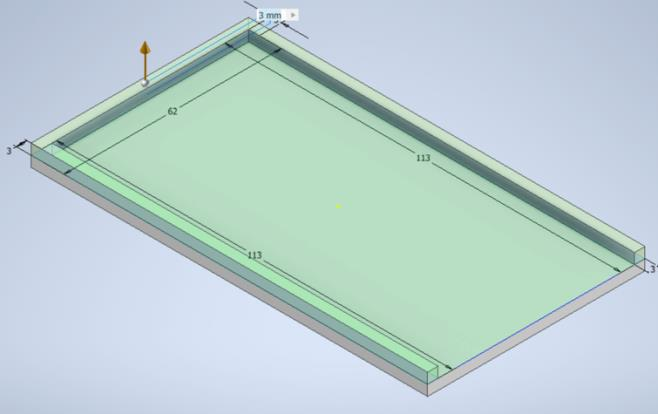
\includegraphics[height=5cm]{images/casing/img32.jpg}
\end{figure}

To finish, we created the male version of the slits in the box to allow the cover only to translate in one direction
\begin{figure}[H]
    \centering
    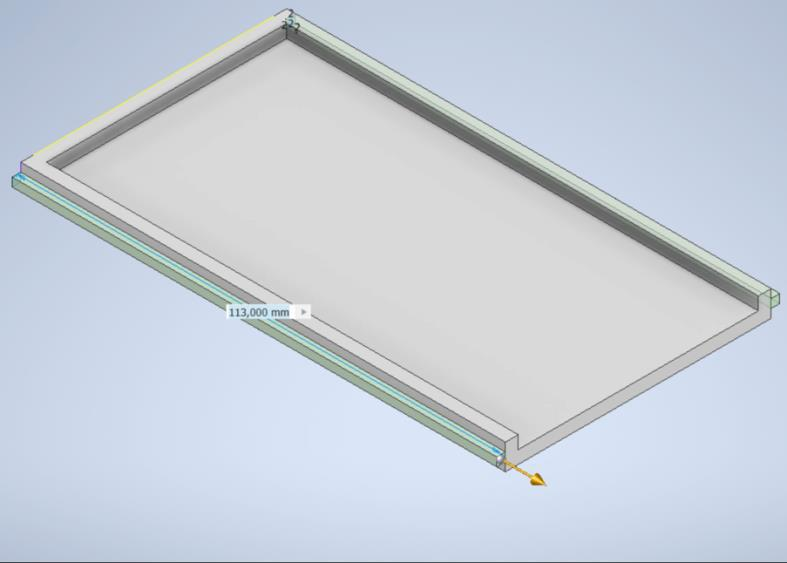
\includegraphics[width=.7\textwidth]{images/casing/img33.jpg}
\end{figure}

\subsection{Nodes Box}
To start with this box, we first created the frame that will receive the components as the Arduino Nano and the sensors. We have to let an opening on the front face of this box to let air pass through it and allow the sensors to get the right values. We also have to let an available place outside the box to place the antenna.
\begin{figure}[H]
    \centering
    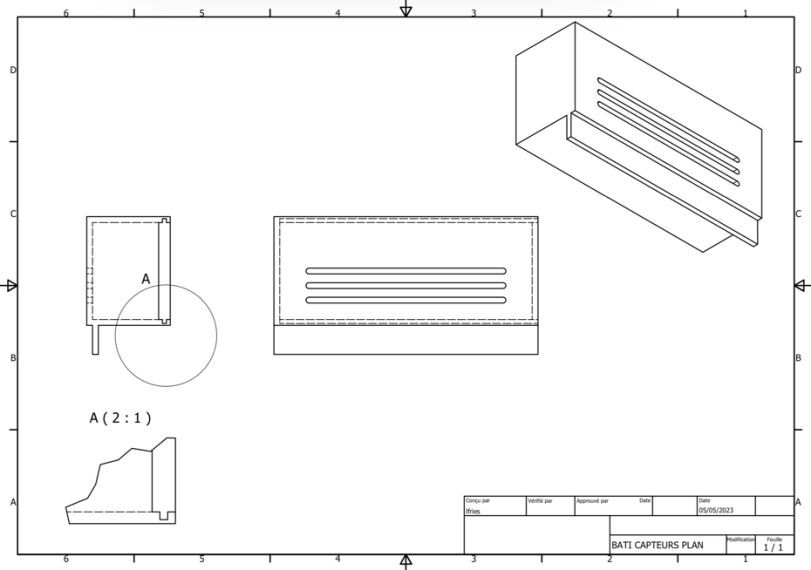
\includegraphics[width=.8\textwidth]{images/casing/img36.jpg}
    \caption{Plan of the box for the node}
\end{figure}

As for the central box, we created a rectangle of the right dimensions to receive the different parts to protect. We gave this rectangle a thickness of 3mm and also created walls to close the sides of the box.
\begin{figure}[H]
    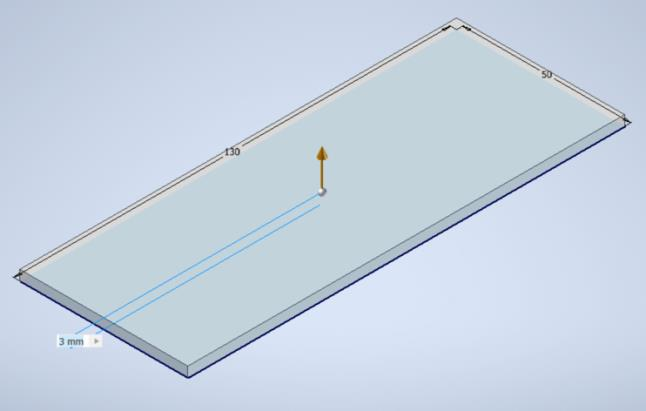
\includegraphics[height=5.5cm]{images/casing/img37.jpg}
    \hfill
    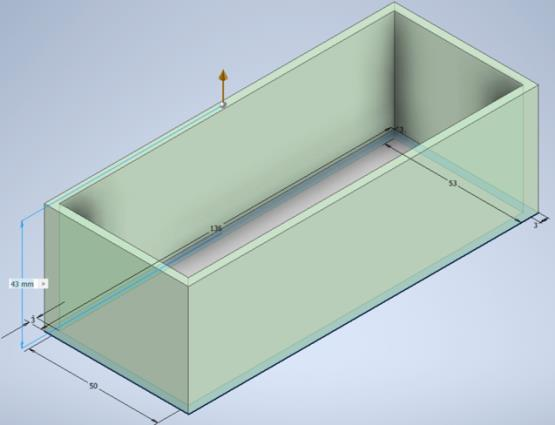
\includegraphics[height=5.5cm]{images/casing/img38.jpg}
\end{figure}

We also created the same slits as the first on the back of this box, in the way to close it with the same type of cover.
\begin{figure}[H]
    \centering
    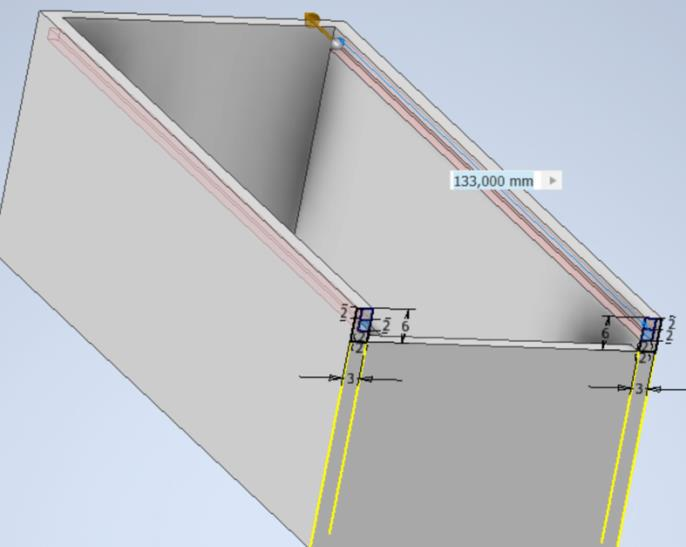
\includegraphics[width=.7\textwidth]{images/casing/img41.jpg}
\end{figure}

Finally, we had to create the openings on the front face and prepare space for the antenna.
\begin{figure}[H]
    \centering
    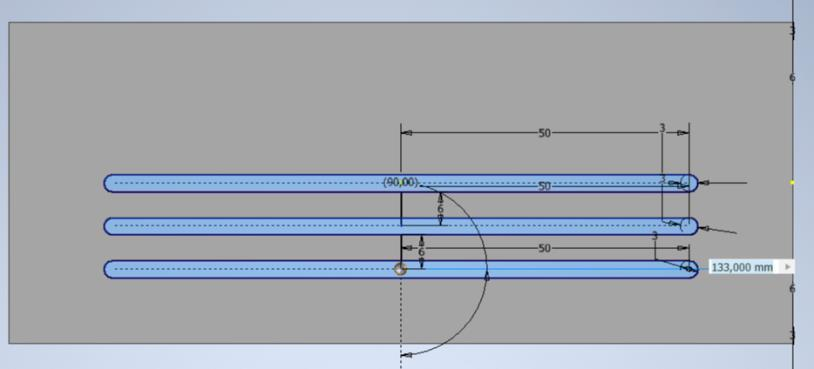
\includegraphics[width=.7\textwidth]{images/casing/img42.jpg}
    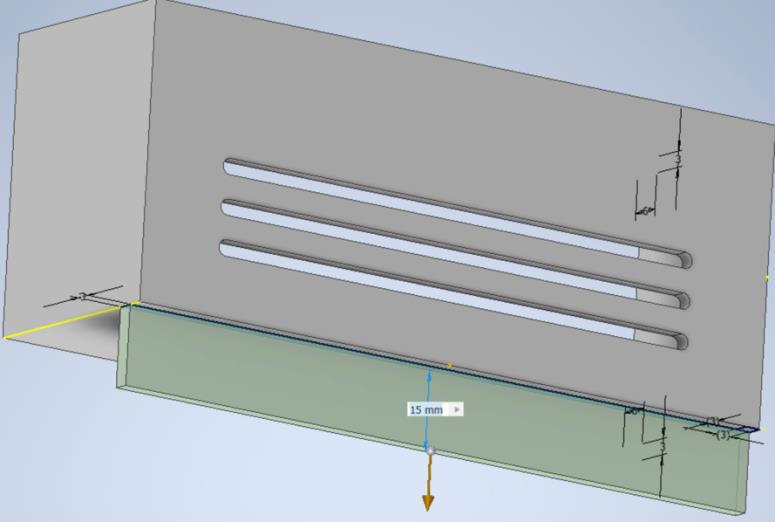
\includegraphics[width=.7\textwidth]{images/casing/img43.jpg}
\end{figure}

To close this box we created the same type of cover as for the first box.
\begin{figure}[H]
    \centering
    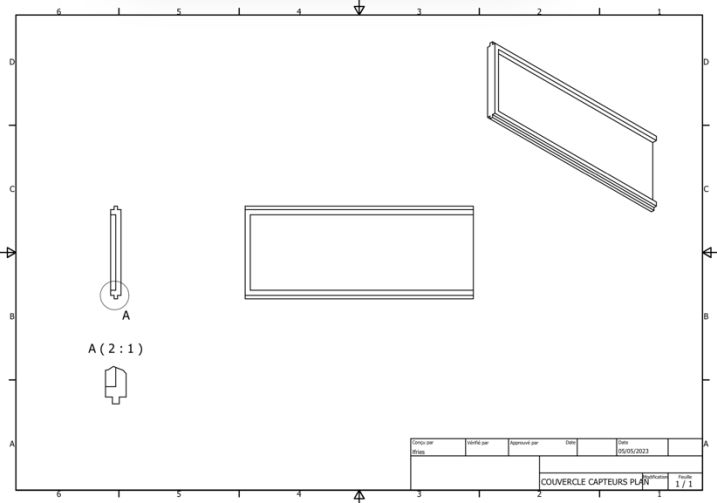
\includegraphics[width=.7\textwidth]{images/casing/img46.jpg}
    \caption{Plan of the cover for the node box}
\end{figure}

\subsection{Remarks}
After the impression and thinking of other problems, like putting the node box outside, we thought about different things that we could have done in another way. \\
--- First, we could have created a little roof on the front face of the node box, so in rainy situations, water wouldn’t really go inside it. \\
--- We also thought that it would have been better if we printed this box in white because, in the case of high temperatures outside, our black box will be hot really fast. \\
--- For both of the boxes, we also tough that we could have created a wall bracket to place our box on the wall with a screw or double-face adhesive.